\documentclass[12pt]{article}
\usepackage[T1]{fontenc}
\usepackage[light,math]{iwona}
\usepackage[latin1]{inputenc}
\usepackage{amsmath}
\usepackage{ulem}
\usepackage{mathtools}
\usepackage{xspace}
\usepackage{xstring}
\usepackage[english]{babel}
\usepackage[font=small,labelfont=bf]{caption}
\usepackage[centering,includeheadfoot,margin=2cm]{geometry}
\usepackage{tikz}
\usepackage{graphicx}
\usetikzlibrary{calc,shapes,arrows,automata,trees,shadows,decorations.pathmorphing,positioning,
shapes.misc,shapes.arrows,chains,matrix,scopes,decorations.pathmorphing,backgrounds}

\begin{document}
\title{CS375 WK8}
\author{Jason N Mansfield}
\maketitle


\begin{center}
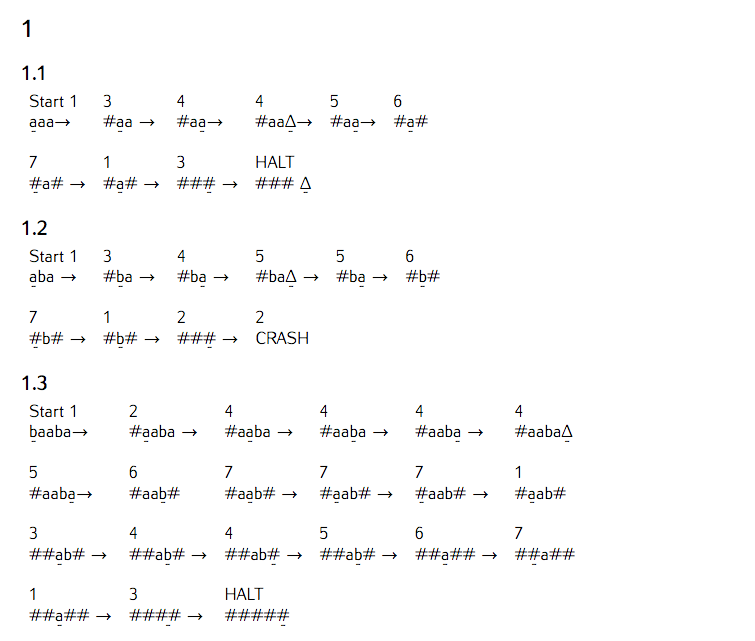
\includegraphics[scale=0.5]{Screen1};
\clearpage
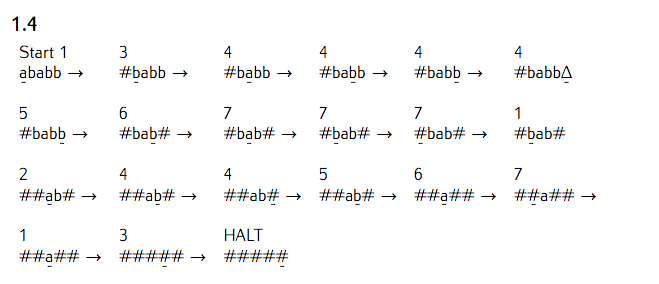
\includegraphics[scale=0.5]{Screen2};
\end{center}
\setcounter{section}{1}
\section{}
The language accepted by this TM is all words with an odd number of letters that have an a as
the middle letter.

\begin{enumerate}
\item[Step 1] This is the Start state but also a state that is always revisited by successful strings for traversal to State 3 which leads to HALT provided the final remaining letter is a. This State also can send strings off to CRASH if the final letter is b. The only acceptable characters are either b or a which are thus replaced with the \# character. This will happen on the left hand side of the string when a return visit to state 1 happens again. Provided this string does not crash or HALT from a single a before hand. This allows the string to be narrow down optimally for a central a as the only remaining character.
\item [Step 2] Either States 2 or 3 are reached at this point. If in fact state 2 is reached a two was read and either the entire string is composed of all \# symbols or $\Delta$ both of which will reach a successful HALT. If the string has a remaining character a or b traversal to state 4 will be next. Regarding state 3, if this state is reach and is entirely composed of \# symbols then the last character read was a b and the machine crashes. 
\item[Step 3] Reaching state 4 the string is read to the right up until either reaching a \# character or $\Delta$ at which point traversal to state 5 is achieved. During traversal the machine moves back one local to the previous character either a or b which allows it to continue on to state 6  replacing this character with a \# symbol and thus narrowing down this string once again. This is of course to add the \# symbol to the right hand side of the string. Between state 6 and back to 1 the tape head is moved to the far left.
\item[Step 4] 
Returning to state one the left hand side of the string can be evaluated for traversal to either 2 or 3. If the string has more than one remaining a or b it will simply replace the next to the last character with \# and loop again. If however the string is on its final character and it is an a the machine will traverse to 3 followed by a successful HALT. If the final character is a b it will traverse to 2 and crash.
\end{enumerate}
\clearpage
\section{}
\subsection{}
\begin{figure}
\begin{center}
\caption{ODDPALINDROME}
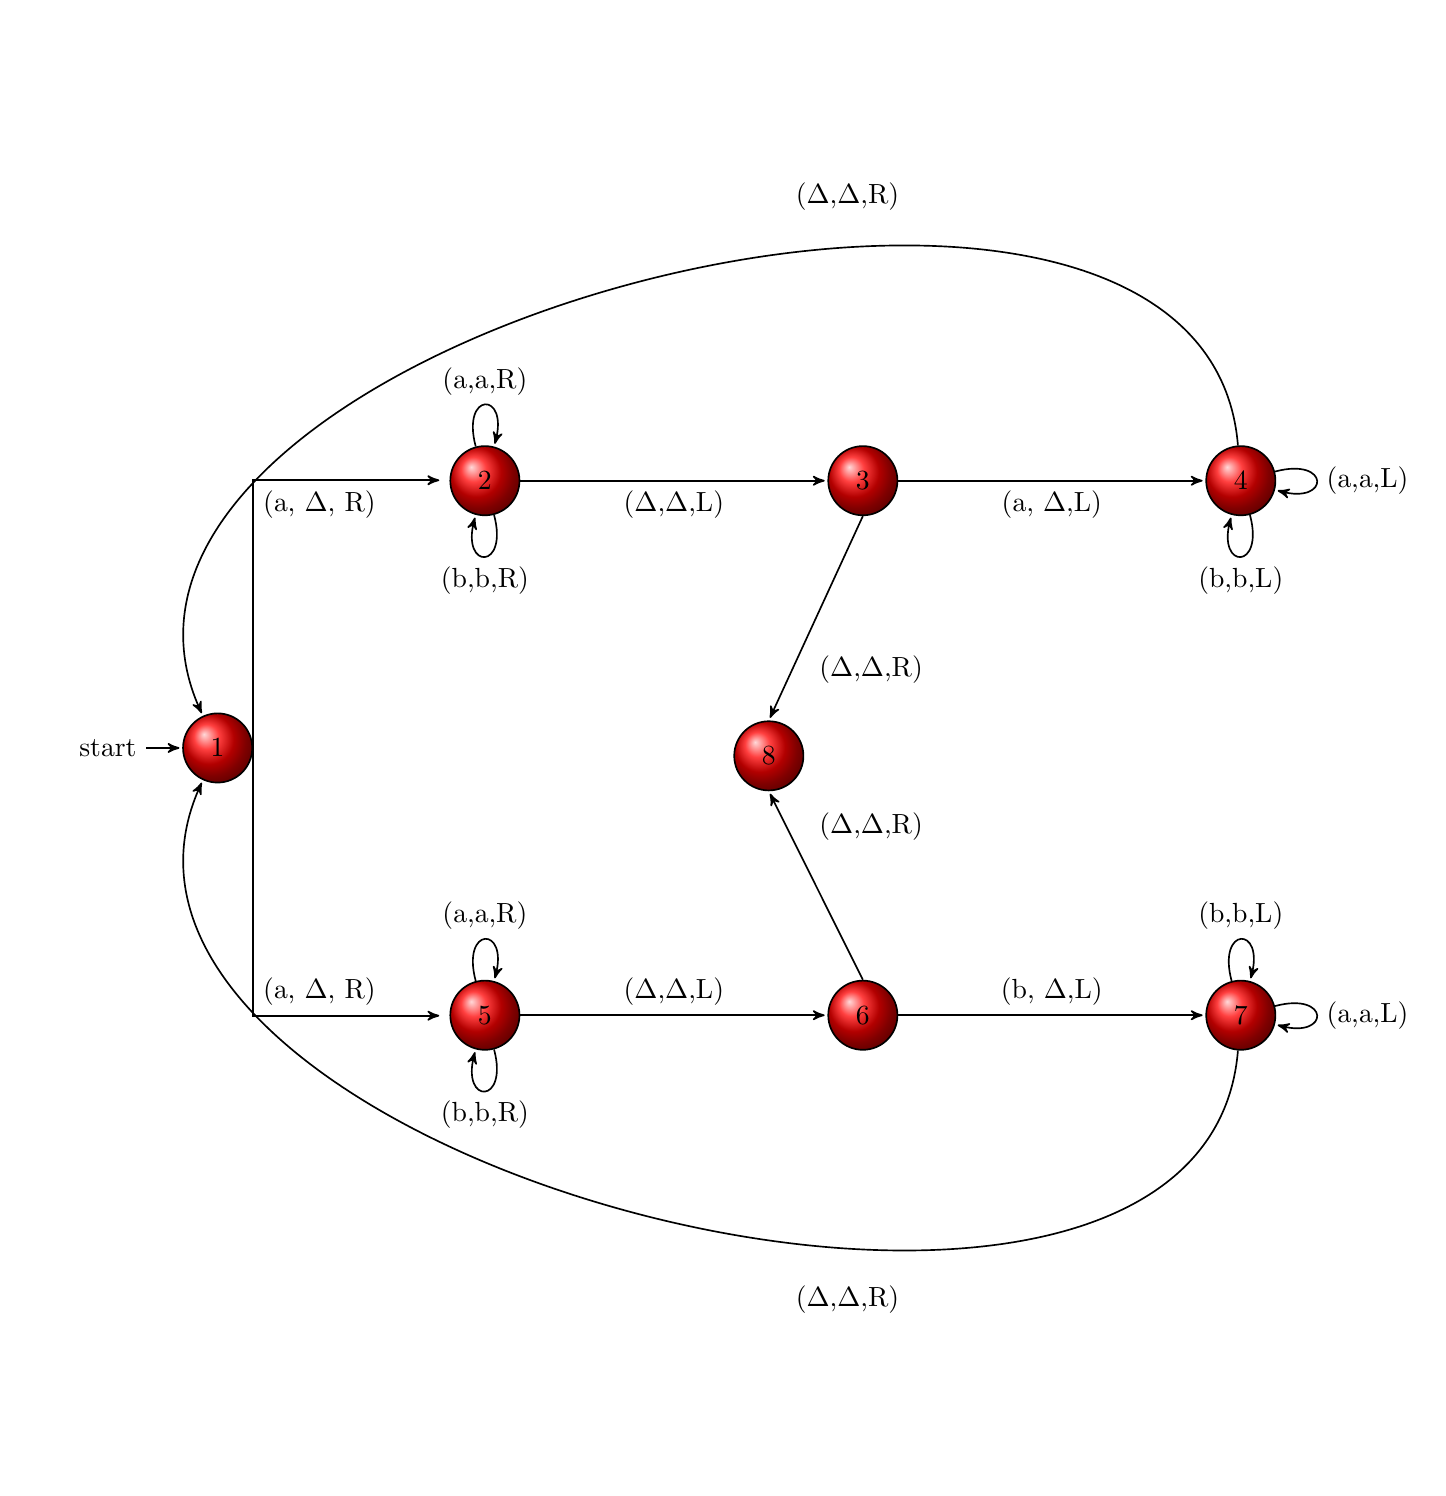
\begin{tikzpicture}[->,>=stealth',shorten >=1pt,auto,node distance=4.8cm, semithick]
\tikzstyle{every state}=[draw=black,text=black, ball color=red]
\node[state,initial](1){1};
\node[state][above right of=1](2){2};
\node[state][right of=2](3){3};
\node[state][right of=3](4){4};
\node[state][below right of=1](5){5};
\node[state][right of=5](6){6};
\node[state][right of=6](7){7};
\node[state]  at (7,-0.1) (8){8};
\node at (8,7) (top) {($\Delta$,$\Delta$,R)};
\node at (8,-7) (floor) {($\Delta$,$\Delta$,R)};
\node at (8.3, 1) (mid-top) {($\Delta$,$\Delta$,R)};
\node at (8.3, -1) (mid-floor) {($\Delta$,$\Delta$,R)};
 %paths
 \path (7) edge [bend left=100]node{}(1);
 \path (4) edge [bend right=100]node{}(1);
\path(2) edge[loop below]node{(b,b,R)}(2);
\path(2) edge[loop above]node{(a,a,R)}(2);
\path(5) edge[loop below]node{(b,b,R)}(5);
\path(5) edge[loop above]node{(a,a,R)}(5);
\path(4) edge[loop below]node{(b,b,L)}(4);
\path(4) edge[loop right]node{(a,a,L)}(4);
\path(7) edge[loop above]node{(b,b,L)}(7);
\path(7) edge[loop right]node{(a,a,L)}(7);
              
 %draw
 \draw [->] ($(1.east)$)  -++(0,3.4) node[below right]{(a, $\Delta$, R)} -++(2.4,3.4);   
 \draw [->] ($(1.east)$)  -++(0,-3.4) node[above right]{(a, $\Delta$, R)} -++(2.4,-3.4);  
 \draw [->] ($(2.east)$)  -l node[below](5a){($\Delta$,$\Delta$,L)} ($(3.west)$); 
 \draw [->] ($(5.east)$)   -l node[above](5a){($\Delta$,$\Delta$,L)} ($(6.west)$); 
  \draw [->] ($(3.east)$)  -l node[below](5a){(a, $\Delta$,L)}  ($(4.west)$); 
 \draw [->] ($(6.east)$)  -l node[above](5a){(b, $\Delta$,L)} ($(7.west)$); 
  \draw [->] ($(3.south)$)  -l ($(8.north)$); 
 \draw [->] ($(6.north)$)  -l ($(8.south)$); 
\end{tikzpicture} 
\end{center}
\end{figure}
\clearpage
\subsection{}
\subsubsection{abbba~Odd~string}
\[
  \overset{1~START}{\b{a}bbba} \rightarrow
   \overset{2}{\b{b}bba}\rightarrow
   \overset{2}{b\b{b}ba}\rightarrow
   \overset{2}{bb\b{b}a}\rightarrow
   \overset{2}{bbb\b{a}}\rightarrow
  \overset{2}{bbba\b{$\Delta$}}\rightarrow
  \overset{3}{bbb\b{a}}\rightarrow
   \overset{4}{bb\b{b}}\rightarrow
   \overset{4}{b\b{b}b}\rightarrow
  \overset{4}{\b{b}bb}
\]

\[
\overset{4}{\b{$\Delta$}bbb}\rightarrow
\overset{1}{\b{b}bb}\rightarrow
\overset{5}{\b{b}b}\rightarrow
 \overset{5}{b\b{b}}\rightarrow
\overset{5}{bb\b{$\Delta$}}\rightarrow
\overset{6}{b\b{b}}\rightarrow
\overset{7}{\b{b}}\rightarrow
\overset{7}{\b{$\Delta$}b}\rightarrow
\overset{1}{\b{b}}\rightarrow
\overset{7}{\b{$\Delta$}}\rightarrow
\overset{6}{\b{$\Delta$}}\rightarrow
\overset{8~HALT}{\b{$\Delta$}}
\]
\subsubsection{bbaaabb~Odd~string}
\[
\overset{1~START}{\b{b}baaabb}\rightarrow
\overset{5}{\b{b}aaabb}\rightarrow
\overset{5}{b\b{a}aabb}\rightarrow
\overset{5}{ba\b{a}abb}\rightarrow
\overset{5}{baa\b{a}bb}\rightarrow
\overset{5}{baaa\b{b}b}\rightarrow
\overset{5}{baaab\b{b}}\rightarrow
\overset{5}{baaabb\b{$\Delta$} }\]

\[
\overset{6}{baaab\b{b}}\rightarrow
\overset{7}{baaa\b{b}}\rightarrow
\overset{7}{baa\b{a}b}\rightarrow
\overset{7}{ba\b{a}ab}\rightarrow
\overset{7}{b\b{a}aab}\rightarrow
\overset{7}{\b{b}aaab}\rightarrow
\overset{7}{\b{$\Delta$}baaab}\rightarrow
\overset{1}{\b{b}aaab}\rightarrow
\overset{1}{\b{a}aab}
\]

\[
\overset{5}{\b{a}aab}\rightarrow
\overset{5}{a\b{a}ab}\rightarrow
\overset{5}{aa\b{a}b}\rightarrow
\overset{5}{aaa\b{b}}\rightarrow
\overset{5}{aaab\b{$\Delta$}}\rightarrow
\overset{6}{aaa\b{b}}\rightarrow
\overset{7}{aa\b{a}}\rightarrow
\overset{7}{a\b{a}a}\rightarrow
\overset{7}{\b{a}aa}\rightarrow
\overset{7}{\b{$\Delta$}aaa}\rightarrow
\overset{1}{\b{a}aa}
\]

\[
\overset{2}{\b{a}a}\rightarrow
\overset{2}{a\b{a}}\rightarrow
\overset{2}{aa\b{$\Delta$}}\rightarrow
\overset{3}{a\b{a}}\rightarrow
\overset{4}{\b{a}}\rightarrow
\overset{4}{\b{$\Delta$}a}\rightarrow
\overset{1}{\b{a}}\rightarrow
\overset{2}{\b{$\Delta$}}\rightarrow
\overset{3}{\b{$\Delta$}}\rightarrow
\overset{8~HALT}{\b{$\Delta$}}
\]

\subsubsection{abba~Even~string}

\[
\overset{1}{\b{a}bba}\rightarrow
\overset{2}{\b{b}ba}\rightarrow
\overset{2}{b\b{b}a}\rightarrow
\overset{2}{bb\b{a}}\rightarrow
\overset{2}{bba\b{$\Delta$}}\rightarrow
\overset{3}{bb\b{a}}\rightarrow
\overset{4}{b\b{b}}\rightarrow
\overset{4}{\b{b}b}\rightarrow
\overset{4}{\b{$\Delta$}bb}\rightarrow
\overset{1}{\b{b}b}
\]

\[
\overset{5}{\b{b}}\rightarrow
\overset{5}{b\b{$\Delta$}}\rightarrow
\overset{6}{\b{b}}\rightarrow
\overset{7}{\b{$\Delta$}}\rightarrow
\overset{1}{\b{$\Delta$}}\rightarrow
\overset{CRASH}{\b{$\Delta$}}
\]

\subsubsection{bbaabb~Even~string}

\[
\overset{1}{\b{b}baabb}\rightarrow
\overset{5}{\b{b}aabb}\rightarrow
\overset{5}{b\b{a}abb}\rightarrow
\overset{5}{ba\b{a}bb}\rightarrow
\overset{5}{baa\b{b}b}\rightarrow
\overset{5}{baab\b{b}}\rightarrow
\overset{5}{baabb\b{$\Delta$}}\rightarrow
\overset{6}{baab\b{b}}\rightarrow
\overset{7}{baa\b{b}}\rightarrow
\overset{7}{ba\b{a}b}\rightarrow
\]

\[
\overset{7}{b\b{a}ab}\rightarrow
\overset{7}{\b{b}aab}\rightarrow
\overset{7}{\b{$\Delta$}baab}\rightarrow
\overset{1}{\b{b}aab}\rightarrow
\overset{5}{\b{a}ab}\rightarrow
\overset{5}{a\b{a}b}\rightarrow
\overset{5}{aa\b{b}}\rightarrow
\overset{5}{aab\b{$\Delta$}}\rightarrow
\overset{6}{aa\b{b}}\rightarrow
\overset{7}{a\b{a}}
\]

\[
\overset{7}{\b{a}a}\rightarrow
\overset{7}{\b{$\Delta$}aa}\rightarrow
\overset{1}{\b{a}a}\rightarrow
\overset{2}{\b{a}}\rightarrow
\overset{2}{a\b{$\Delta$}}\rightarrow
\overset{3}{\b{a}}\rightarrow
\overset{4}{\b{$\Delta$}}\rightarrow
\overset{1}{\b{$\Delta$}}\rightarrow
\overset{CRASH}{\b{$\Delta$}}
\]
\end{document}
